\subsection{Comparison}

In this section we compare the results and approach from \cite{shitov2020sublinear} and \cite{kwan2020extension} by working out general similarities or differences. We further look at how both bounds are achieved numerically (in an asymptotic view). In the end we examine how the proofs could be altered to use them in the other's setting.

We start with a quick overview of both results:

\begin{itemize}
  \item \cite{shitov2020sublinear} proves Theorem~\ref{theorem:xc}, which states that every $n$-gon $P$ has $\xc(P) \in O(n^{2/3})$.
  \item \cite{kwan2020extension} proves Theorem~\ref{theorem:cyclic-xc}, which states that every cyclic $n$-gon $P$ has $\xc(P) \in O(n^{1/2})$.
\end{itemize}

First we list the general similarities of both approaches:

\begin{itemize}
  \item Both follow the strategy of splitting the polygon into smaller slices.\\
        \cite{shitov2020sublinear} splits the original polygon into $12$ slices, each $\pi/6$-thin, which are treated separately.\\
        \cite{kwan2020extension} splits the polygon into $O(n^{1/2})$ arcs containing $O(n^{1/2})$ vertices. But here they are treated as a whole.

  \item There is some notion of enclosing vertices in both.\\
        \cite{shitov2020sublinear} requires an envelope around vertices in its central theorem \ref{theorem:gluing}. It is used to build an extended formulation for this specific polygon.\\
        \cite{kwan2020extension} uses a ``lampshade argument'', which builds a polygon around vertices away from a set of facets, to show that a slice of the slack matrix has constant nonnegative rank.
\end{itemize}

Even though some ideas are common to both methods, they are more different than similar:

\begin{itemize}
  \item One key difference is the type of approach:\\
        \cite{shitov2020sublinear} uses a purely geometric method.\\
        \cite{kwan2020extension} uses the linear-algebraic strategy using slack matrices for its main reasoning. But lemmata are often proved geometrically. The approach has the advantage that transformation on the slack matrix, which don't alter the nonnegative rank, can not always be represented geometrically.

  \item There is another difference in how they treat subsets of vertices:\\
        \cite{shitov2020sublinear} iteratively extracts a large subsequence with small extension complexity (ignoring all other vertices).\\
        \cite{kwan2020extension} splits its consideration by constantly many colors, but always handles the dependencies to either all other vertices or all other facets.
\end{itemize}

We go on analyzing numerically how each approach ends up with its asymptotical bound.

$\xc(P) \in O(n^{2/3})$ for arbitrary $n$-gons $P$ in \cite{shitov2020sublinear}:
\begin{itemize}
  \item There is a subsequence $u$ with $m \in O(n^{2/3})$ vertices for every $n$-gon, for which the main theorem can be applied asymptotically optimal.
  \item It provides the bound $\xc(u) \in O(m^{1/2}) = O(n^{1/3})$ for the extension complexity of that subsequence.
  \item Iteratively extracting such a subsequence $u$ proves the bound $\xc(P) \in O(n^{2/3})$.
\end{itemize}

$\xc(P) \in O(n^{1/2})$ for cyclic $n$-gons $P$ in \cite{kwan2020extension}:
\begin{itemize}
  \item We split the circle into $\abs{\X} \in O(n^{1/2})$ arcs.
  \item We split the slack matrix into $O(1)$ ``color columns''.
  \item From these we build a matrix $K$ with $\rank_+ K \in O(\abs{\X_c})$, where $\X_c$ are the arcs of color $c$.
  \item Each ``color column'' in the slack matrix has $\rank_+ M[V,F_c] \in O(\abs{\X_c} + n^{1/2})$.
  \item Joining these columns results in $\rank_+ M \in O(\abs{\X} + n^{1/2}) = O(n^{1/2})$.
\end{itemize}

Finally, we have a look at, how each procedure could be used in the other's setting:

\begin{itemize}
  \item Even though the authors of \cite{kwan2020extension} state that \cite[Lemma~10.2]{kwan2020extension} is "the only place where we use this assumption that $P$ is cyclic", the definition of well-separateness uses arc-distance. Generalizing the proof requires something like a boundary-distance, where the distance between two vertices is the sum of the lengths of the edges separating them. In this setting, a counterexample for \cite[Lemma~10.2]{kwan2020extension} can be found easily, because well-separated facets and vertices can still have small slacks (see Figure~\ref{fig:cyclic-counter-example}).\\
        We conclude that this approach can't be adopted easily for the general case, since it relies on $P$ being cyclic in central parts. Still, the used methods may be of value for future approaches.
  \item If we want to improve the bound achieved in \cite{shitov2020sublinear} for cyclic polygons, we have to find a larger subsequence for which we can apply Theorem~\ref{theorem:gluing} optimally. In the best case, we can find a subsequence with $\Theta(n)$ vertices, where $\abs{V},\abs{S},\delta \in \Theta(n^{1/2})$ in Theorem~\ref{theorem:gluing}. Then we could get the same upper bound of $O(n^{1/2})$ for the extension complexity.
\end{itemize}

\begin{figure}[ht]
  \centering
  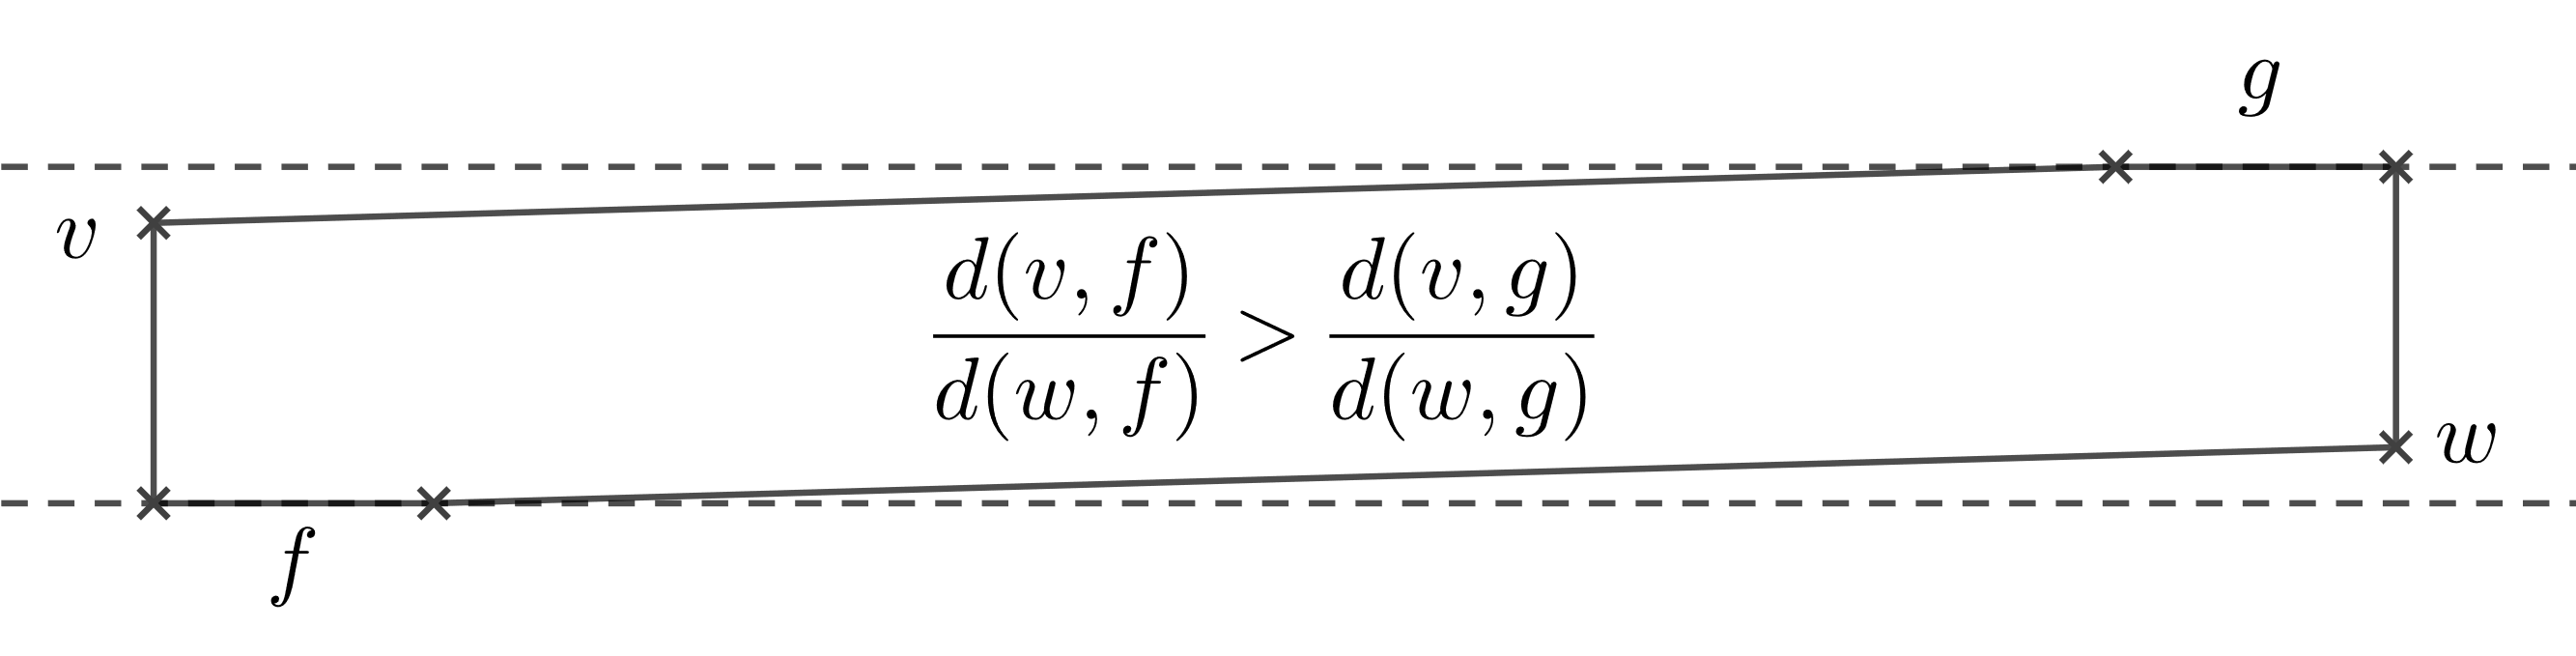
\includegraphics[width=100mm]{cyclic-counter-example.png}
  \caption{Counterexample for \cite[Lemma~10.2]{kwan2020extension}, if it didn't require $P$ to be cyclic.}
  \label{fig:cyclic-counter-example}
\end{figure}
